\begin{activity} \label{A:10.3.8} 
  Shown below in Figure \ref{F:10.3.activity.contour} is a contour
  plot of a function $f(x,y)$ with the value of $f$ labeled on the
  contours.  The point $(2,1)$ is highlighted in red. 

\begin{figure}[ht]
  \begin{center}
    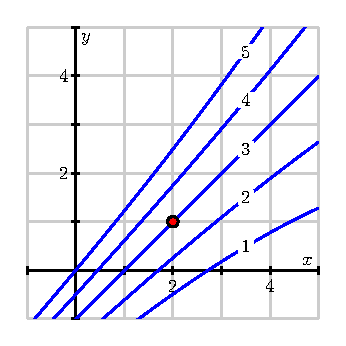
\includegraphics{figures/fig_10_3_activity_contour.eps}
    \caption{A contour plot of $f(x,y)$.}
    \label{F:10.3.activity.contour}
  \end{center}
\end{figure}

\ba
\item Estimate the partial derivatives $f_x(2,1)$ and $f_y(2,1)$.
\item Determine whether the second order partial derivative
  $f_{xx}(2,1)$ is positive or negative, and explain your thinking.
\item Determine whether the second order partial derivative
  $f_{yy}(2,1)$ is positive or negative, and explain your thinking.
\item Determine whether the second order partial derivative
  $f_{xy}(2,1)$ is positive or negative, and explain your thinking.
\item Determine whether the second order partial derivative
  $f_{yx}(2,1)$ is positive or negative, and explain your thinking.
\item Consider a function $g(x,y)$ for which $g_x(2,2) > 0$ and
  $g_{xx}(2,2) < 0$.  Sketch possible behavior of some contour
  lines around $(2,2)$ on the left axes in Figure \ref{F:10.3.activity.grad}.
  \begin{figure}[ht]
    \begin{center}
      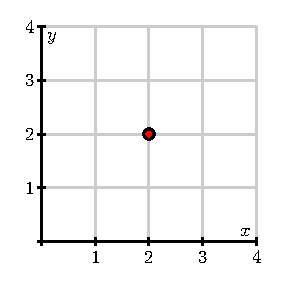
\includegraphics{figures/fig_10_2_activity_grad.eps}
      \hspace*{1in}
      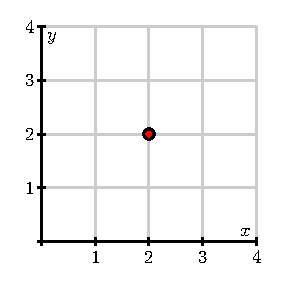
\includegraphics{figures/fig_10_2_activity_grad.eps}
    \end{center}
    \caption{Plots for contour lines of $g$ and $h$.}
    \label{F:10.3.activity.grad}
  \end{figure}
\item Consider a function $h(x,y)$ for which $h_x(2,2) > 0$ and
  $h_{xy}(2,2) < 0$.  Sketch possible behavior of some contour
  lines around $(2,2)$ on the right axes in Figure \ref{F:10.3.activity.grad}.

    
\ea

\end{activity}
\aftera
